\chapter{Non-parametric estimation of regression function using the kernel method}
\section{Introduction}
One can estimate what input was applied to a dynamic Hammerstein system using so called kernel functions.
Assuming as before:
\begin{equation}
    \hat{R}(u) = \frac{\hat{g}(u)}{\hat{f}(u)} =   \frac{\Sigma_{i=1}^{N} y_k K( \frac{u_k-u}{h}) }{   \Sigma_{i=1}^{N} K( \frac{u_k-u}{h}) }
\end{equation}
Where $K(\cdot)$ is a kernel function, which only takes into account local samples to estimate local behaviour.\\
For the sixth laboratory class this method will be used to estimate the regression function of a Hammerstein system.
There were 2 linearities to approximate, depending on which group we were assigned to, and the one estimated in this rapport is the right one.

%% nonlinearities
\begin{figure}[h!]
\begin{center}
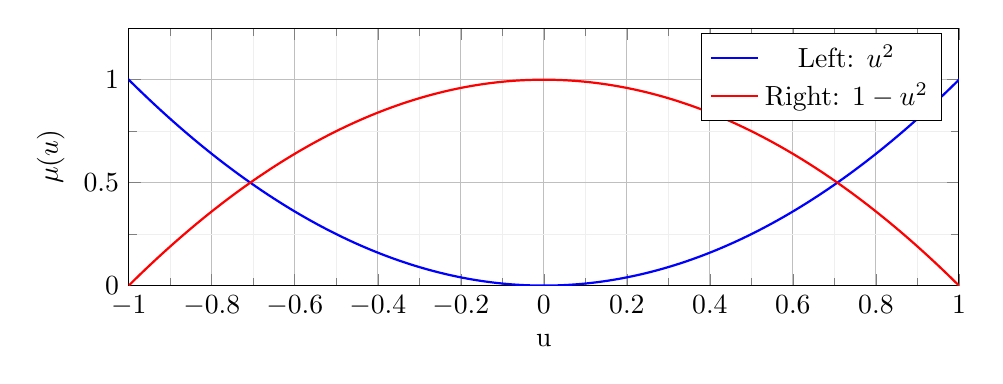
\begin{tikzpicture}
\begin{axis}[
    xmin = -1, xmax = 1,
    ymin = 0, ymax = 1.25,
    grid = both,
    minor tick num = 1,
    major grid style = {lightgray},
    minor grid style = {lightgray!25},
    width = \textwidth,
    height = 0.40\textwidth,
    xlabel = u,
    ylabel = $\mu(u)$]

    \addplot[
        domain = -1.2:1.2,
        samples = 500,
        thick,
        blue,
        ] 
        {
        (x*x)
        };


    \addplot[
        domain = -1:1,
        samples = 500,
        thick,
        red,
        ] 
        {
        (x > -1)*(x < 1)*(1-x*x)
        };
    \legend{
        Left: $u^{2}$,
        Right: $1 - u^{2}$,
        }
\end{axis}
\end{tikzpicture}
\end{center}
\label{app_fig}
\caption{The input functions given to their respective groups}
\end{figure}
\section{Laboratory}
The dynamics of the system are described by the following recurrence relation:
\begin{equation}
    y_k = \frac{1}{2}y_{k-1} + \mu(u_k)
\end{equation}
The task then is to determine what $\mu(u)$ is based only on a set of input output pairs $(u_k,y_k)$. What we'll have to be satisfied with however, is determining what  $\mu(u)$ is up to a shift in value, and a multiplication by different constants. In fact, if we note that:
\begin{equation}
    y_k = \Sigma_{i=0}^{\infty}\gamma_i\mu(u_{k-i})
\end{equation}
We can rewrite $R(u)$ as:
\begin{equation}
    R(u) = E\left\{ \gamma_0\mu(u_k)  +  \Sigma_{i=1}^{\infty}\gamma_i\mu(u_{k-i}) \right\} = \gamma_0\mu(u) + c
\end{equation}
Where c is the expected value of the tail, which can be written as:
\begin{equation}
    c = E \Sigma_{i=1}^{\infty}\gamma_i\mu(u_{k-i}) = \Sigma_{i=1}^{\infty}\gamma_iE\mu(u_{k-i}) = \bar{\mu}(\cdot) \Sigma_{i=1}^{\infty}\gamma_i
\end{equation}
The mean value of the non-linear input function can be determined to be $\bar{\mu} = \frac{2}{3}$. The coefficients $\gamma_i$ can be found from the recurrence relation to be  $\gamma_i = (\frac{1}{2})^{-i}$, which then by a well known result from mathematical analysis gives the value of their infinite sum as 1 - note that the series starts at i = 1 - which finally gives $c = \frac{2}{3}$. This, combined with $\gamma_0 = 1$, tells us that we should expect our estimated $\hat{\mu(\cdot)}$ to be close to $\mu{\cdot} + \frac{2}{3}$.
\\
At least 2 different types of kernel functions had to be investigated during the laboratory, and each will be discussed separately first.
\subsection{The rectangular kernel}
The rectangular kernel can be described as the difference of 2 step functions shifted from each other. Intuitively, it can be understood as a way to calculate only a local mean, with what local exactly means depending on the value of h.

%% plot
\subsection{Dependence on h}

If we plot the difference between the actual input, vs the estimated input, we can see that this difference does indeed oscillate around 0.66. Higher values of h lead to smoother functions, but larger overall errors, especially at the boundaries. Smaller h leads to higher oscillations, but less overall error. With the way the code was implemented, if h is small enough, in relation to the sample size, divisions by 0 can occur.



%% plot approx plot error

\begin{figure}[h!]
\begin{center}
\begin{tikzpicture}
\begin{axis}[
    xmin = -1, xmax = 1,
    ymin = 0, ymax = 1.8,
    grid = both,
    minor tick num = 1,
    major grid style = {lightgray},
    minor grid style = {lightgray!25},
    width = 0.45\textwidth,
    height = 0.50\textwidth,
    xlabel = u,
    ylabel = $\mu(u)$,
    scaled x ticks=false]
    \addplot[
        domain = -1.0:1.0,
        samples = 500,
        thick,
        blue,
        ] 
        {
        1-x*x
        };



    \addplot[color=blue,
        ]
        table [col sep=space, x index = 0, y index=1]{./plot_data/chapter_5/rect_app.dat};

    \addplot[color=green,
        ]
        table [col sep=space, x index = 0, y index=2]{./plot_data/chapter_5/rect_app.dat};

    \addplot[color=red,
        ]
        table [col sep=space, x index = 0, y index=3]{./plot_data/chapter_5/rect_app.dat};

    \addplot[color=orange,
        ]
        table [col sep=space, x index = 0, y index=4]{./plot_data/chapter_5/rect_app.dat};

    \legend{
        $1-u^{2}$,
       $h = 0.001$,
        $h = 0.01$,
        $h = 0.1$,
        $h = 1$}
\end{axis}
\end{tikzpicture}
\begin{tikzpicture}
\begin{axis}[
    xmin = -1, xmax = 1,
    ymin = 0.5, ymax = 1.2,
    grid = both,
    minor tick num = 1,
    major grid style = {lightgray},
    minor grid style = {lightgray!25},
    width = 0.45\textwidth,
    height = 0.5\textwidth,
    xlabel = u,
    ylabel = $\varepsilon$,
    scaled x ticks=false]

    \addplot[color=blue,
        ]
        table [col sep=space, x index = 0, y index=1]{./plot_data/chapter_5/rect_err.dat};

    \addplot[color=green,
        ]
        table [col sep=space, x index = 0, y index=2]{./plot_data/chapter_5/rect_err.dat};

    \addplot[color=red,
        ]
        table [col sep=space, x index = 0, y index=3]{./plot_data/chapter_5/rect_err.dat};

    \addplot[color=orange,
        ]
        table [col sep=space, x index = 0, y index=4]{./plot_data/chapter_5/rect_err.dat};

    \legend{
        $h = 0.001$,
        $h = 0.01$,
        $h = 0.1$,
        $h = 1$}
\end{axis}
\end{tikzpicture}
\caption{Estimations using the rectangular kernel on the left, and their differences with the original input on the right
}
\end{center}
\end{figure}



\subsection{The Gaussian kernel}
The Gaussian kernel works similarity to the rectangular kernel. With the Gaussian function however being smooth and continuous everywhere, we get a different effect from just a simple local mean. Here, the samples far away get gradually less and less relevant to the local behaviour. This continuity leads to smoother functions overall



\begin{figure}[h!]
\begin{center}
\begin{tikzpicture}
\begin{axis}[
    xmin = -1, xmax = 1,
    ymin = 0, ymax = 1.8,
    grid = both,
    minor tick num = 1,
    major grid style = {lightgray},
    minor grid style = {lightgray!25},
    width = 0.45\textwidth,
    height = 0.50\textwidth,
    xlabel = u,
    ylabel = $\mu(u)$,
    scaled x ticks=false]
    \addplot[
        domain = -1.0:1.0,
        samples = 500,
        thick,
        blue,
        ] 
        {
        1-x*x
        };



    \addplot[color=blue,
        ]
        table [col sep=space, x index = 0, y index=1]{./plot_data/chapter_5/gauss_app.dat};

    \addplot[color=green,
        ]
        table [col sep=space, x index = 0, y index=2]{./plot_data/chapter_5/gauss_app.dat};

    \addplot[color=red,
        ]
        table [col sep=space, x index = 0, y index=3]{./plot_data/chapter_5/gauss_app.dat};

    \addplot[color=orange,
        ]
        table [col sep=space, x index = 0, y index=4]{./plot_data/chapter_5/gauss_app.dat};

    \legend{
        $1-u^{2}$,
       $h = 0.001$,
        $h = 0.01$,
        $h = 0.1$,
        $h = 1$}
\end{axis}
\end{tikzpicture}
\begin{tikzpicture}
\begin{axis}[
    xmin = -1, xmax = 1,
    ymin = 0.5, ymax = 1.2,
    grid = both,
    minor tick num = 1,
    major grid style = {lightgray},
    minor grid style = {lightgray!25},
    width = 0.45\textwidth,
    height = 0.5\textwidth,
    xlabel = u,
    ylabel = $\varepsilon$,
    scaled x ticks=false]

    \addplot[color=blue,
        ]
        table [col sep=space, x index = 0, y index=1]{./plot_data/chapter_5/gauss_err.dat};

    \addplot[color=green,
        ]
        table [col sep=space, x index = 0, y index=2]{./plot_data/chapter_5/gauss_err.dat};

    \addplot[color=red,
        ]
        table [col sep=space, x index = 0, y index=3]{./plot_data/chapter_5/gauss_err.dat};

    \addplot[color=orange,
        ]
        table [col sep=space, x index = 0, y index=4]{./plot_data/chapter_5/gauss_err.dat};

    \legend{
        $h = 0.001$,
        $h = 0.01$,
        $h = 0.1$,
        $h = 1$}
\end{axis}
\end{tikzpicture}
\caption{Estimations using the Gaussian kernel on the left, and their differences with the original input on the right}
\end{center}
\end{figure}




\subsubsection{Dependence on h}
Similar observations can be made here as in the case of the rectangular kernel. With the obvious difference that the function is overall much smoother, and no division by 0 can ever occur.


\section{Conclusions}

Both kernels perform adequately. To use either of them effectively an appropriate h must be chosen, not large enough to induce unnecessary errors, but not small enough to produce large oscillations. 


